\chapter{Related Work}
\label{chapter:relatedwork}

\section{Related Work}

Facial expressions have an important role in human communication, specially about transmitting emotions. With the crescent development of computer vision techniques in artificial intelligence, a lot of effort has been dedicated in recognising facial expression.

\begin{figure}[!htb]	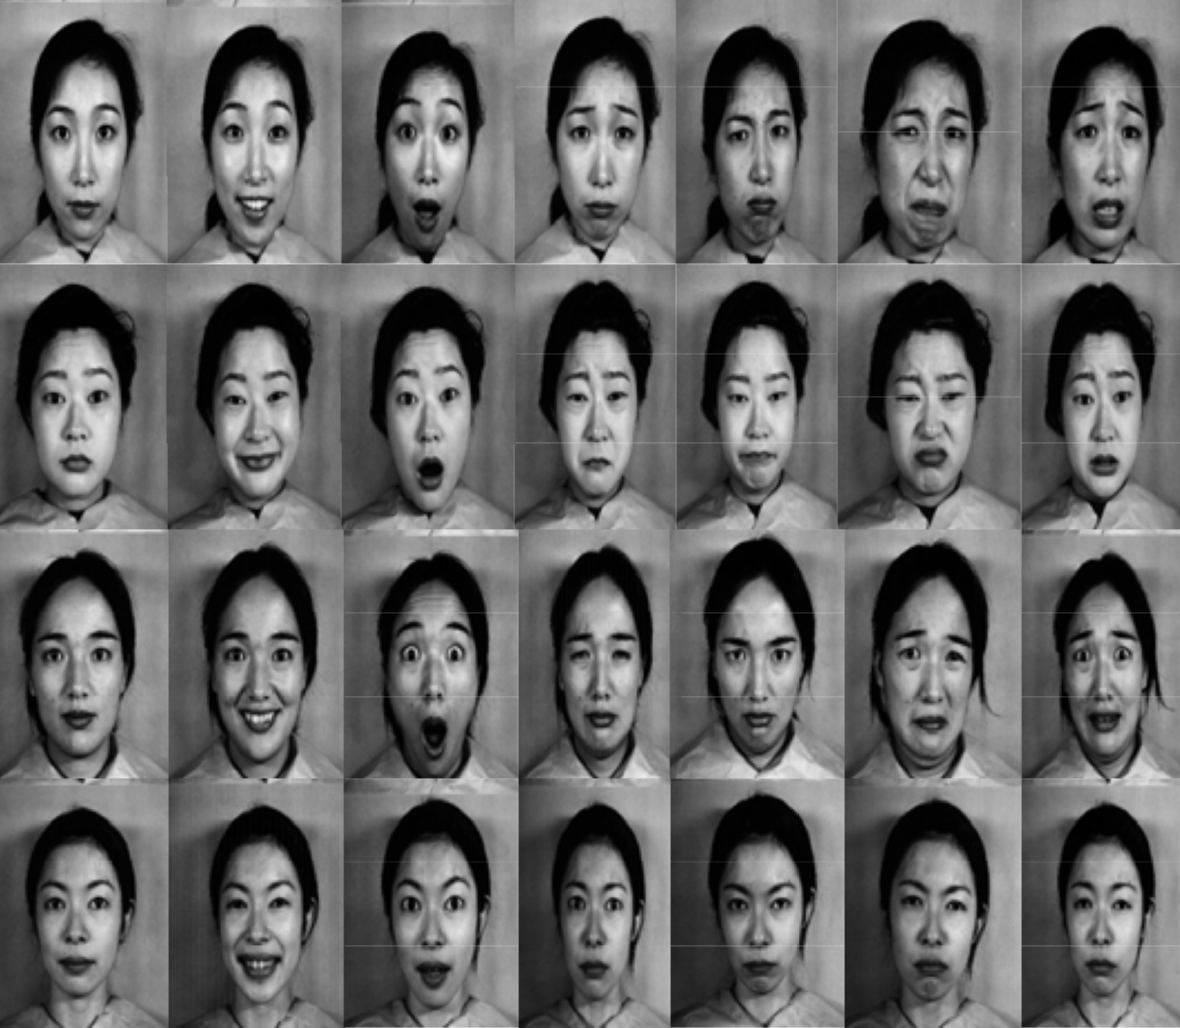
\includegraphics[width=0.9\textwidth]{images/jaffe.png} 
    \centering

\caption{
Facial expression samples from JAFFE \cite{LyonsCodingWavelets} database. Figure Taken from \cite{Sarode2010FacialRecognition}
} 

\label{fig:facial_expressions}
\end{figure}

A common theme in recognition of facial expression of emotions is the use of multimodal approaches.  This section shows some of the approaches that has been presented in the recent years. Different approaches have been used in multimodality, some by utilizing visual modalities obtained from the face or some using another source of information different from the visual information. Using different modalities can give a boost to performance by giving additional complementary information. According to literature recognition of affective emotions consists of four steps: face detection, face registration, feature extraction and expression recognition. 

Some of the methods used for face detection are Viola and Jones \cite{ViolaRapidFeatures}, convolutional neural networks (CNN) \cite{Dalal2005HistogramsDetection} and support vector machines (SVM) over HOG features \cite{Osadchy2007SynergisticModels}. Then, for face segmentation, some use it to extract the face and thus reduce the search space \cite{VijayLakshmi2010SegmentationTechniques}; also, some authors proposed more advanced techniques such as face correction and background elimination among other techniques. 

After the face has been detected, many expression recognition authors detect fiducial points such as face expressions. Some authors have proposed to rotate the face or frontalize the face to make it easier to detect expressions. Different authors proposed different approaches depending if the problem is using greyscale, RGB, infrared or any other modality. This process is normally called face alignment and has become important for improving accuracy in expression recognition.

Since some of these efforts uses multimodal approaches, a fusion of such inputs is necessary. There are different possible ways in which data can be joined depending on the stage that they are fuse. One possible way is to use two-stream architecture that can fuse spatial and temporal information \cite{Feichtenhofer2016ConvolutionalRecognition}. Another fusion strategy is middle fuse, this strategy combines different modalities in the intermediate layers \cite{Neverova2016ModDrop:Recognition}.

%%%%%%%%%%%%%%%%%%%
% SUBSECTION: RGB
%%%%%%%%%%%%%%%%%%%
\subsection{RGB Emotion Recognition}

%%%% CK+ %%%%
\subsubsection{Cohn-Kanade}
Originally presented by Kanade et al. \cite{KanadeComprehensiveAnalysis}, the Cohn-Kanade (CK) database is intended for detecting individual facial emotion-specified expression. It was later extended into the CK+ by Lucey et al. \cite{LuceyTheExpression}. These two datasets uses 7 basic emotion categories: Anger, Contempt, Disgust, Fear, Happy, Sadness and Surprise; and 30 facial action units (AUs) that represent contractions of a specific set of
facial muscles.

\begin{figure}[!htb]	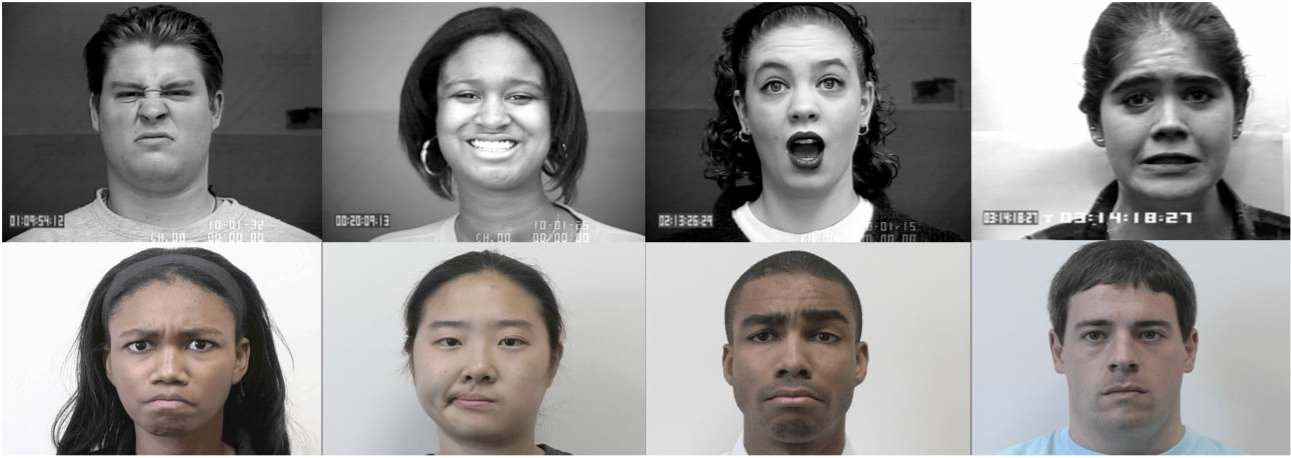
\includegraphics[width=0.9\textwidth]{images/CK+.png} 
    \centering

\caption{
The images on the top level are from the original CK database and those on the bottom are from the CK+database. Both dataset present 7 emotions and 30 AUs.
} 

\label{fig:ck}
\end{figure}

%%%% AAM %%%%
\subsubsection{Active Appearance Model}
Kanade et al. propose an Active Appearance Model (AAM) to track the face and extract features. AAMs align a pre-defined linear shape model to a previously unseen source image containing the object of interest. In other words, AAMs fit their shape and appearance components. The features obtained are similarity-normalized shape (SPTS) and canonical appearance (CAPP). Then, they use a linear classifier, a support vector machines (SVMs) for identifying the facial expressions and emotions \cite{KanadeComprehensiveAnalysis}.

\begin{figure}[!htb]	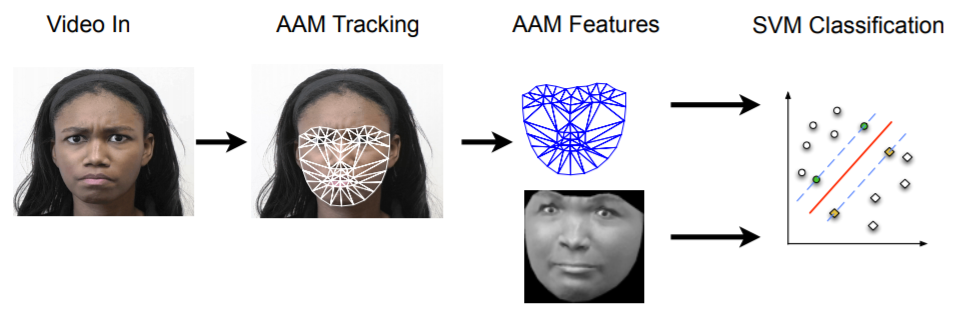
\includegraphics[width=0.9\textwidth]{images/aam.png} 
    \centering

\caption{
The face is tracked using an AAM and some features are obtained. These features are used for classification using a linear SVM.
} 

\label{fig:aam}
\end{figure}

%%%% DISFA %%%%
\subsubsection{Denver Intensity of Spontaneous Facial Action}
DISFA (Denver intensity of spontaneous facial action) is a dataset for facial expression recognition proposed by Mavadati et al. DISFA roughly contains 130,000 annotated frames from 27 adult participants. For every video frame, the intensity of 12 action unit (AUs) was manually annotated. The AUs found in the dataset are the most common in emotion expression that have been used in computer vision previously \cite{Mavadati2013DISFA:Database}.

\begin{figure}[!htb]	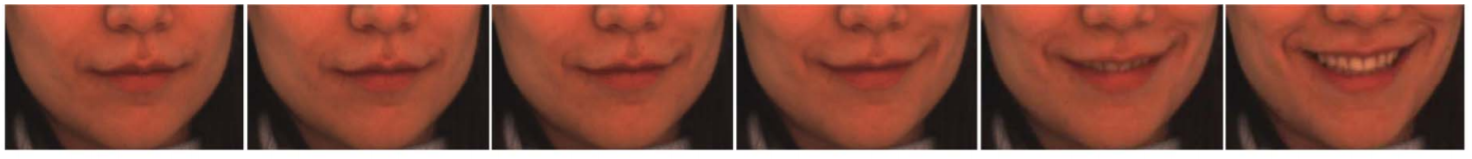
\includegraphics[width=0.8\textwidth]{images/DISFA.png} 
    \centering

\caption{Sample facial images with AU \cite{Mavadati2013DISFA:Database} } 

\label{fig:disfa}
\end{figure}

Mavadati et al. propose a model consisting of extracting features from cropped images. The features chosen by them are local binary pattern histogram (LBPH), histogram of oriented gradient (HOG), and localized Gabor features. Then the features were reduced from high dimensionality using nonlinear manifold learning, which assumes that low-dimensional features are embedded in a high dimensional space. To extract these low-dimensional features of facial images, the Laplacian Eigenmap followed by spectral regression (SR) technique is used. Finally, they trained SVM classifier adapted for multi-class classification. 

%%%%%%%%%%%%%%%%%%%
% SUBSECTION: MULTI-MODAL
%%%%%%%%%%%%%%%%%%%
\subsection{Multi-modal Emotion Recognition}
Another approach to emotion recognition in literature is the use of multi-modal. This means that the dataset not only uses one modality, which RGB is the most common, but uses more data inputs to recognise facial expressions for emotion recognition. 

%%%% NVIE %%%%
\subsubsection{Natural Visible and Infrared Facial Expression}
The Natural Visible and Infrared Facial Expression database (NVIE) was introduced by Wang et al \cite{Wang2010AInference}. The dataset contains visible and thermal videos recorded simultaneously. All images are categories into six categories: happiness, sadness, surprise, fear, anger, and disgust. 

\begin{figure}[!htb]	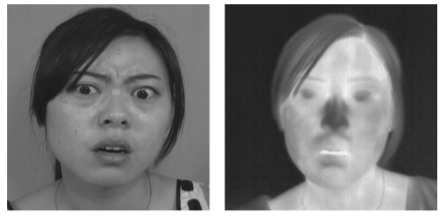
\includegraphics[width=0.6\textwidth]{images/infrared.png} 
    \centering

\caption{
Visual and Infrared image of a subject side by side.
} 

\label{fig:infrared}
\end{figure}

Using the NVIE dataset, Liu et al. \cite{LiuSPONTANEOUSDESCRIPTOR} present a model using both thermal and visual videos. Their approach uses fisher vector aggregated by local and global trajectory features. Gaussian mixture models are constructed based on the features extracted. 

\begin{figure}[H]	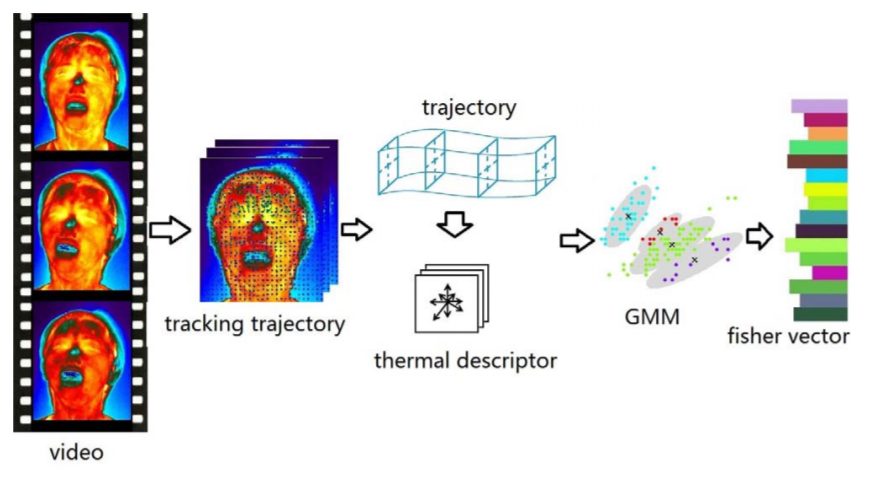
\includegraphics[width=0.6\textwidth]{images/thermal.png} 
    \centering

\caption{
Overview of the model proposed by Liu et al. \cite{LiuSPONTANEOUSDESCRIPTOR}
} 

\label{fig:thermal}
\end{figure}

%%%%%%%%%%%%%%%%%%%
% SUBSECTION: DEEP LEARNING
%%%%%%%%%%%%%%%%%%%
\subsection{Deep Learning Emotion Recognition}
Deep Architectures have started to be used in extensively in the recent years since they have proven to be really successful and have outranked previous state of the art approaches. These deep architectures have overcome the limitations by taking into account non-linear feature interactions.

%%%% emoFBVP %%%%
\subsubsection{emoFBVP}
Ranganathan et al. introduced the emoFBVP database of multimodal recordings. The multi-modality consists of face, body gesture, voice and physiological signals. The participants displayed 23 different emotions, each emotion with three different intensities. Next, they propose a Convolutional Deep Belief Model (CDBN) for emotion recognition using this dataset \cite{RanganathanMultimodalArchitectures}.

\begin{figure}[!htb]	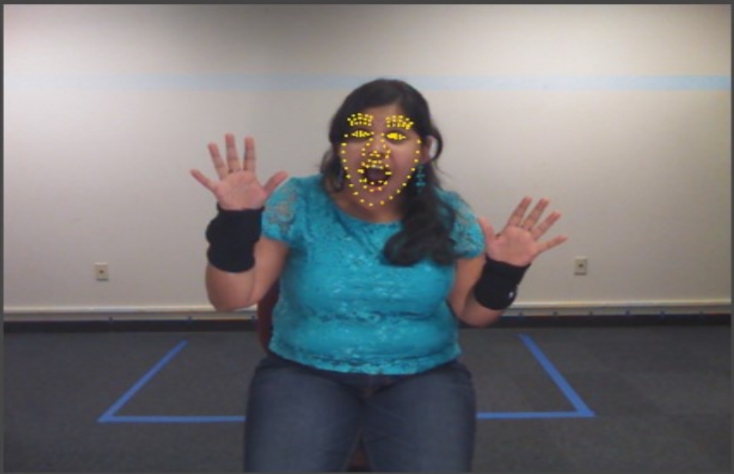
\includegraphics[width=0.7\textwidth]{images/emoFBVP.png} 
    \centering

\caption{
Example of a surprise emotion in emoFBVP dataset.
} 

\label{fig:emoFBVP}
\end{figure}

Convolutional Restricted Boltzmann Machines (CRBMs) are an extension of Restricted Boltzmann Machines (RBMs). Stacking convolutional RBM together, they form a convolutional deep belief network. CDBNs are generative models that are trained layer-wise. The last layer of CRBMs is a matrix, that has spatial proximity of the pixels, these makes learning features more robust. The model proposed by Ranganathan et al. uses the features obtained by the last layer of the CDBN has an an input in a SVM.

%%%% KDEF %%%%
\subsubsection{Karolinska Directed Emotional Faces}
A pre-trained deep CNN as a Stacked Convolutional AutoEncoder (SCAE) is presented by Ruiz-Garcia et al. The SCAE is trained in a greedy layer-wise unsupervised way. The model is trained using the Karolinska
Directed Emotional Faces (KDEF) dataset for emotion recognition by means of facial expressions images \cite{Ruiz-GarciaStackedExpressions}. The participants in KDEF dataset show the emotions; sad, surprised, neutral, happy, fear, disgust, and angry. All the faces are centred, both mouth and
eyes are fixed in a specified coordinate.

\begin{figure}[!htb]	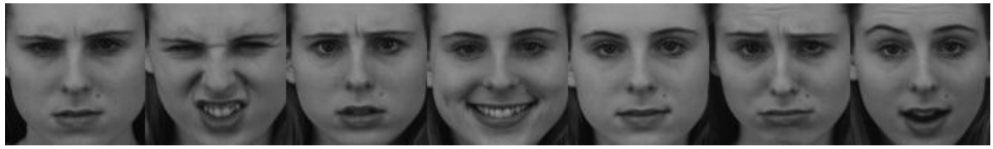
\includegraphics[width=0.9\textwidth]{images/KDEF.png} 
    \centering

\caption{
Participant of the KDEF database showing the emotions: angry, disgust, fear, happy, neutral, sad and surprise.
} 

\label{fig:KDEF}
\end{figure}

The first step is to pre-train a CNN model, with only four convolutional layers, as a SCAE. Each block of layers is used as a component of the Auto-Encoder that replaces Max Pooling with Upsampling layers. After the Auto-Encoders have been trained, the weights for each are put together as a Stacked Convolutional Auto-Encoder. The full model architecture is shown in figure \ref{fig:stacked}.

\begin{figure}[H]	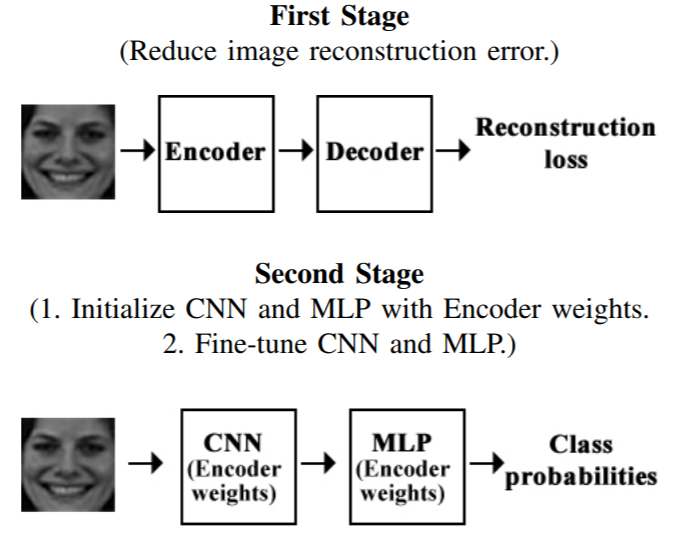
\includegraphics[width=0.6\textwidth]{images/stacked.png} 
    \centering

\caption{
SCAE architecture.
} 

\label{fig:stacked}
\end{figure}

%%%%%%%%%%%%%%%%%%%
% SUBSECTION: AUTHENTICITY
%%%%%%%%%%%%%%%%%%%
\subsection{Authenticity of Hidden Emotions}

Accuracy of deception judgments

Reading between the lies identifying concealed and falsified emotions in universal facial expressions

Intelligent expressions of emotions